\chapter{Recommendations}
Recommendation for future research is first of all the filtered of static devices, as this could improve the quality of the results. Furthermore additional research is required to find methods that can be used for determining the quality of the results, especially concerning the movement from and to the campus.

The detail of the data could be improved by increasing the frequency with which the eduroam system is scanning. This could especially support analysis on the use of different entrances. With the present frequency of one scan round per 5 minutes it is highly likely that the first scan when someone is entering a building is not at the entrance. Detail on which routes are travelled between buildings and validating movement from and to the campus could possible be accomplished by strategically placed scanners outdoor. Finally it is recommended to store the locations of access points digitally in a single map. This would support the process of identification of movement patterns inside buildings. 

Finally caution should be taken with the dataset regarding people their privacy. It is relatively easy to identify a particular user and track that person via the data.

\section{Entrances and exits}\label{entrances and exists}
% Xander

This section will describe the undergoing process in order to know how frequent the entrances and exits of a building are used. Knowing this will give insight into the use of a building, the spatial context and the relation between these two. Our hypothesis is that access points located near the entrance(s) of a building are most frequently used as first access point when entering a building, and as last access point when leaving a building. Firstly, an approach will be presented that does not take in account that devices might get scanned when passing by the building. In the second approach we will make use of the pre-processed data which excludes the devices that get scanned when passing by the building. 

\subsection{First approach:including devices passing by}
The first approach makes use of the raw wifilog data, by finding the part in a sequence in which a device is scanned by an access point in a building and is subsequently scanned in another building. With the location of the access points known, we hope to get insight into the use of an entrance or exit location in a building. 
\begin{figure}[H]
\centering
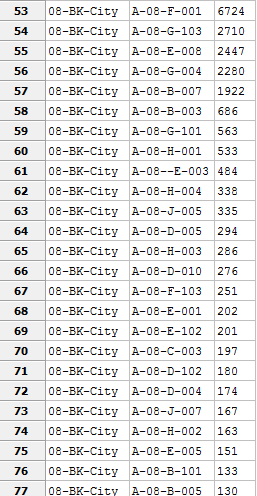
\includegraphics[scale=0.45]{entrances_firstapproach_bk}
\captionsetup{justification=centering}
\caption{A segment of the resulting table after querying}
\label{figure:Entrance1ApproachTable}
\end{figure}

The stays in which the device is scanned once are not filtered out. These single scans imply that a person with the device only passed by the building, thus was not really located in the building. 

\begin{figure}[H]
\centering
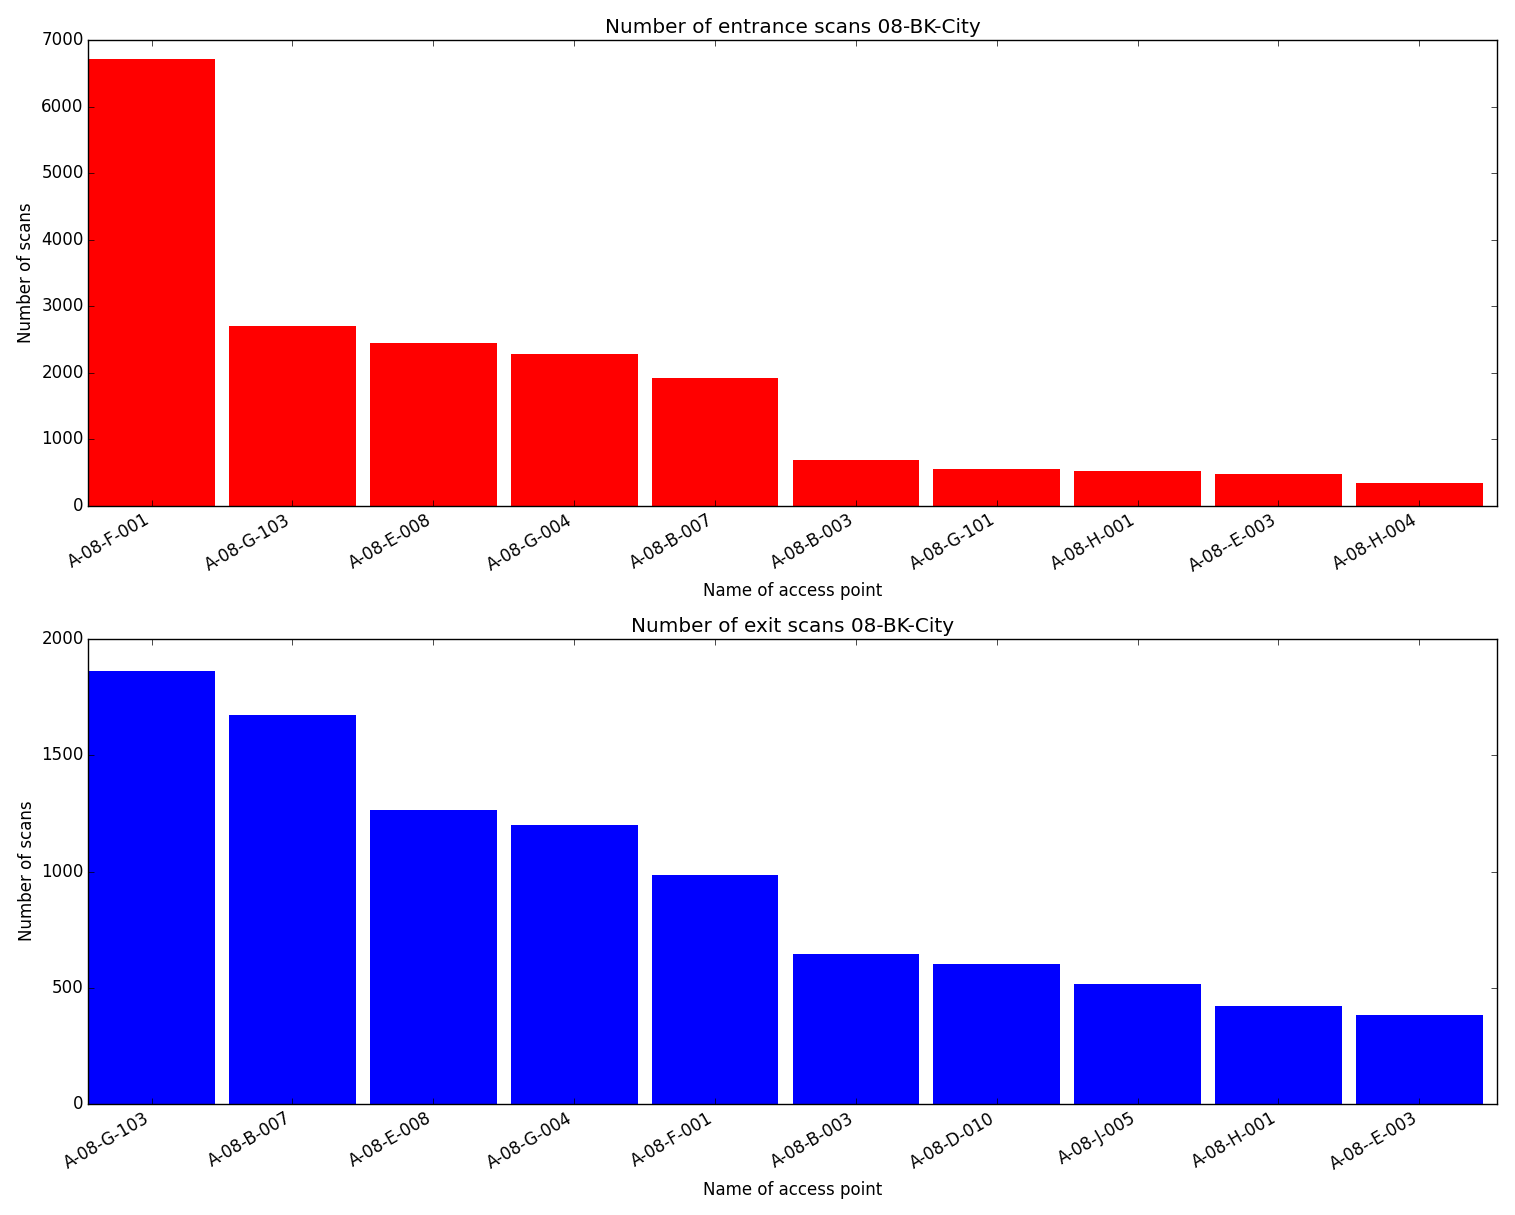
\includegraphics[scale=0.25]{entrances_firstapproach}
\captionsetup{justification=centering}
\caption{Most frequently used entrance and exit access points in BK-City}
\label{figure:Entrance1Approachfigure}
\end{figure}

In order to know whether these access points(see \autoref{figure:Entrance1Approachfigure}) are located near an entrance, the access point maps of BK-City is used. The access point maps are the building plans enriched with the location of each wifi access point installed in the building. Currently, the access point maps of BK-City are the only ones available. Looking at the location of the access points with the highest frequency, gives an interesting result (\autoref{figure:Entrance1Approachaploc}).
 
\begin{figure}[H]
\centering
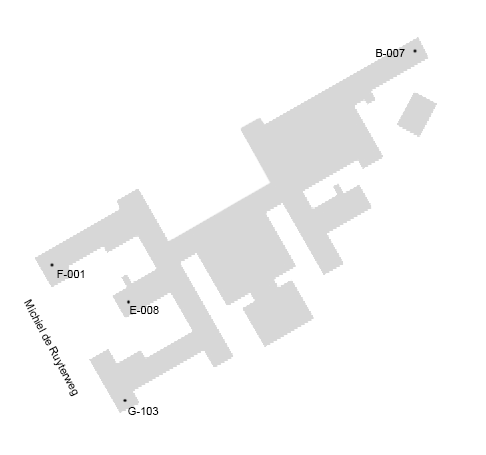
\includegraphics[scale=0.7]{entrances_aplocs_firstapproach}
\captionsetup{justification=centering}
\caption{The location of the most frequently used entrance and exit access points}
\label{figure:Entrance1Approachaploc}
\end{figure}
Most of the frequently used access points are located at the western part of BK-City (\autoref{figure:Entrance1Approachaploc}). Also, there is no entrance or exit located near most of these access points. Knowing that lots of people are passing in the street next to the western part of the building, we can conclude the result of this analysis is distorted due not filtering out the devices that get scanned when passing by the building.

\subsection{Second approach:excluding devices passing by}\label{secondapproach}

\autoref{figure:Entrance2Approachtable} depicts the table as a result of the pre-processing as described in \autoref{preprocessing}. The records represent the stays for each mac, including the first and last access points (ap\_ start and ap\_ end).

\begin{figure}[H]
\centering
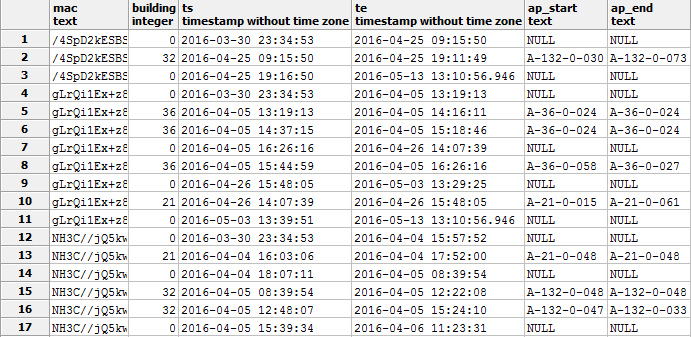
\includegraphics[scale=0.6]{entrances_secondapproach_table}
\captionsetup{justification=centering}
\caption{A segment of the table as a result of the pre-processing}
\label{figure:Entrance2Approachtable}
\end{figure}

The table also includes 'world' (in the \autoref{figure:Entrance2Approachtable} represented by NULL) which implies the device is not located on the campus. 

The following simple SQL statement is used to plots the most frequently used entrance access points.

\begin{lstlisting}[language=SQL]
SELECT ap_start, count(*)
FROM table
GROUP BY ap_start
ORDER BY count desc;
\end{lstlisting}	

Ap\_ end is used, instead of ap\_ start, for plotting the most frequently used exit access points in a building.

\begin{figure}[H]
\centering
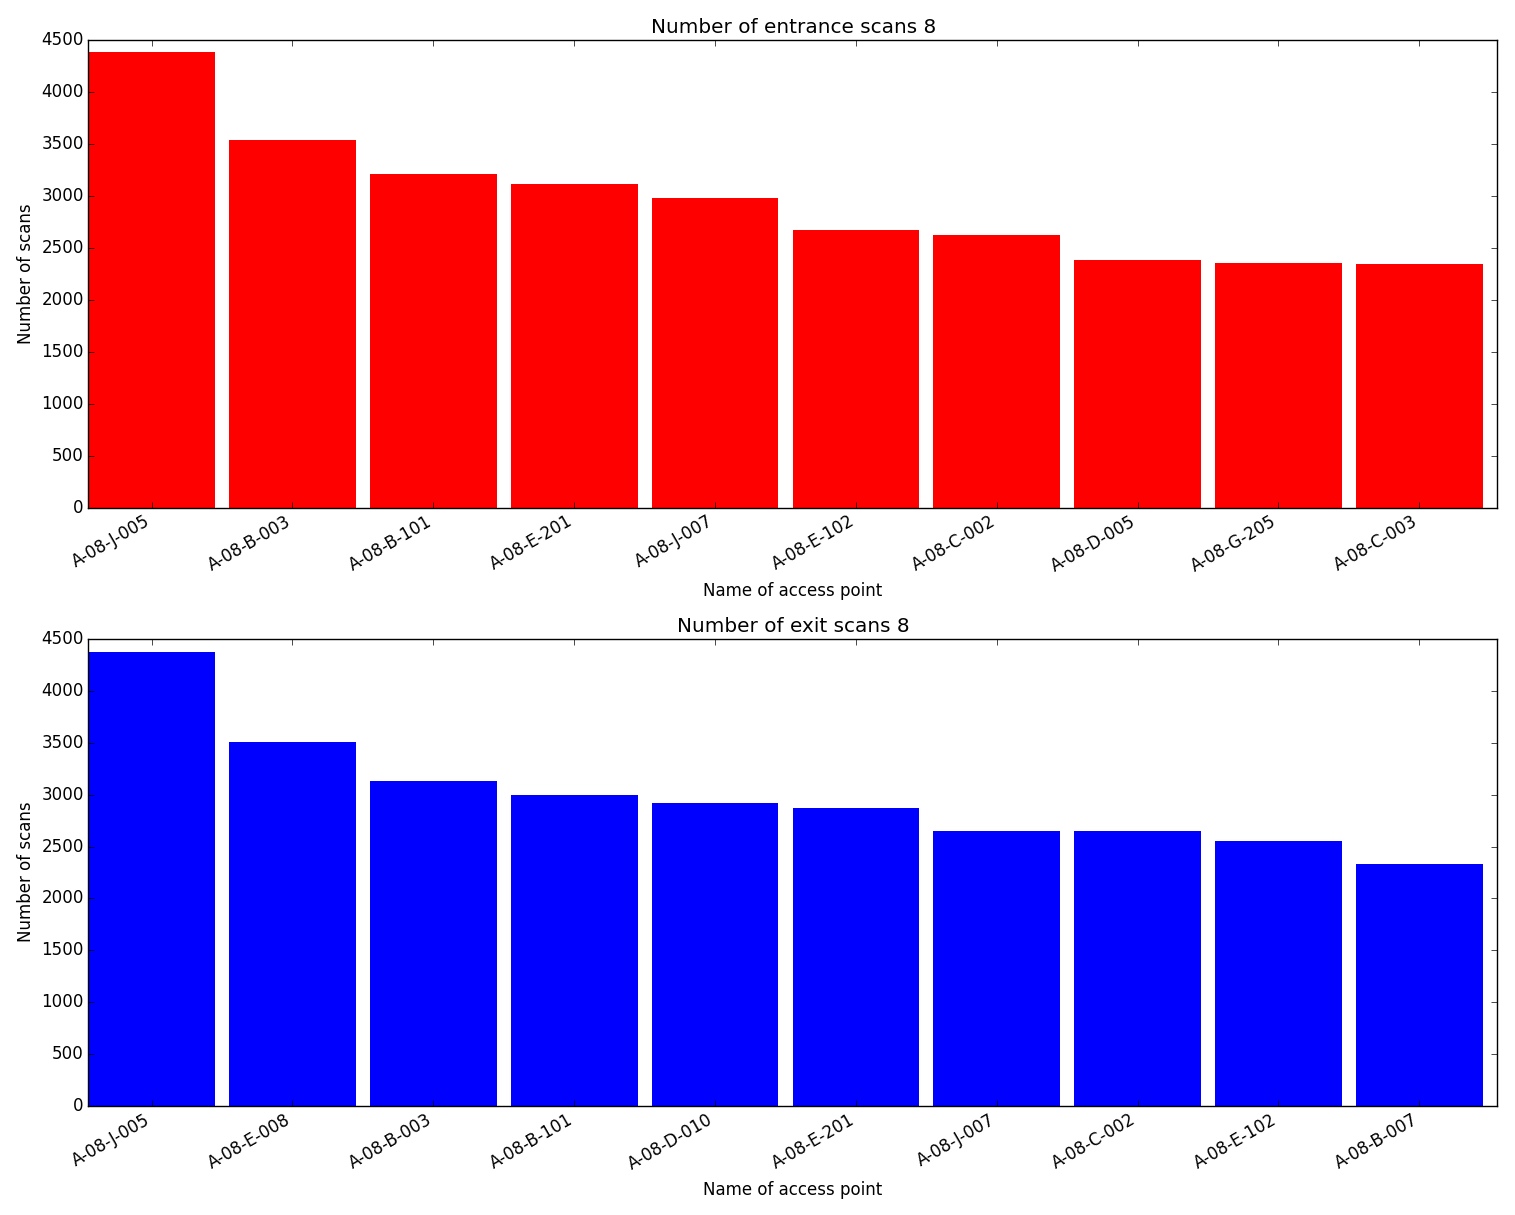
\includegraphics[scale=0.32]{entrances_secondapproach}
\captionsetup{justification=centering}
\caption{The most frequently used entrance and exit access point for BK-City
}
\label{figure:Entrance2Approach}
\end{figure}

The most frequently used access point, A-08-J-005, is not located near an entrance or exit (see \autoref{figure:Entrance2Approach}). This is different than expected. Although it is not very logical in the first place, it still might be one of the first or last access points a device connects with. The reason for this is that the A-08-J-005 access point is placed in in an open space without many objects that could block the wifi signals.

\begin{figure}[H]
\centering
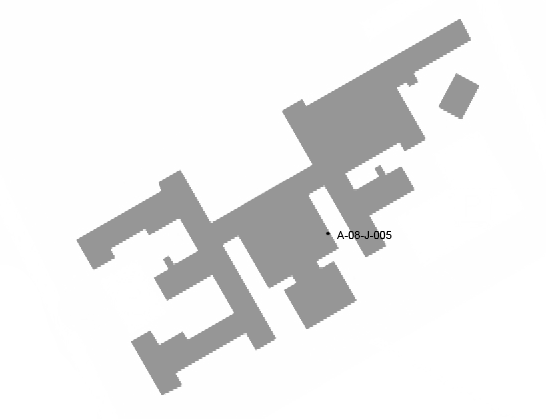
\includegraphics[scale=0.6]{map_ap1_secondapproach}
\captionsetup{justification=centering}
\caption{The location of the most frequently used entrance and exit access point, according to our second approach
}
\label{figure:Entrance2Approachaploc}
\end{figure}

We expected the access point to be located much closer to an entrance or exit. The plan is to set up an experiment in order to justify the unexpected result. In this experiment we will check to what access points different devices (laptops and mobile phones) connect when entering or leaving a building.

\subsection{Frequency of entrance and exit access points}
This section will describe the analysis on the frequency of entrance and exit access points. As described in \autoref{secondapproach}, the most frequently used entrance and exit access points are not always are located near an entrance or exit. Though it is still possible to analyze how frequent these access point are used. The results will be aggregated, meaning it represents more than a single day.

\textbf{Entering}
First we will take a closer look at an access point which appears to be one of the first that scans the device. This will be A-08-J-005 in BK-City, see \autoref{figure:Entrance2Approach} in \autoref{secondapproach}. The chart below shows the frequency of entrance access point A-08-J-005 for devices entering BK-city, over a 24 hour time period. 

\begin{figure}[H]
\centering
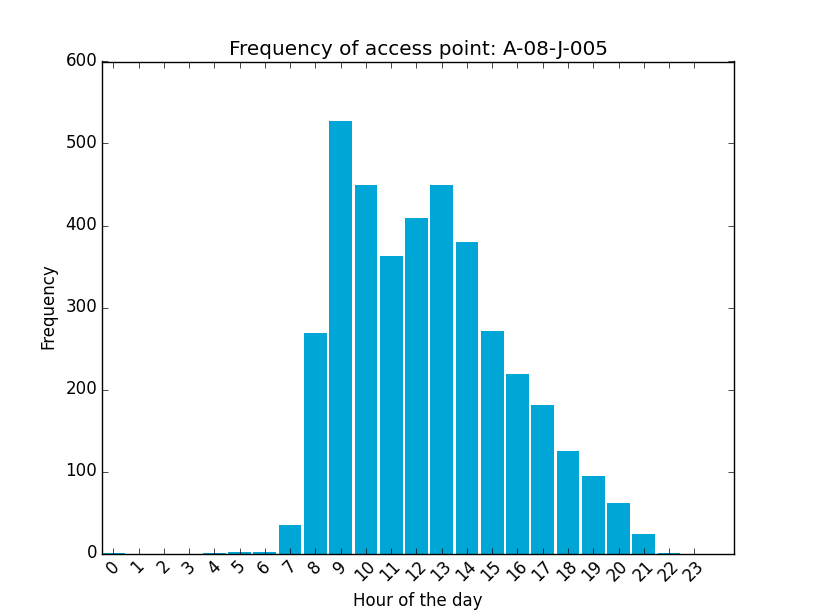
\includegraphics[scale=0.5]{entrances_frequency_secondapproach}
\captionsetup{justification=centering}
\caption{Frequency of entrance access point A-08-J-005
}
\label{figure:A-08-J-005Entrance}
\end{figure}

The chart shows two peaks; in the morning and around 12pm to 1pm. This is in line with what we expected. In the morning a large group enters the building and around 12pm to 1 pm a large group enters the building after the lunch break. 

\textbf{Exiting}

For the exit situation, again the A-08-J-005 access point will be used. This access point also appears to be the most frequently used exit access points. The chart below depicts the frequency of devices leaving the building over a 24 hour period.

\begin{figure}[H]
\centering
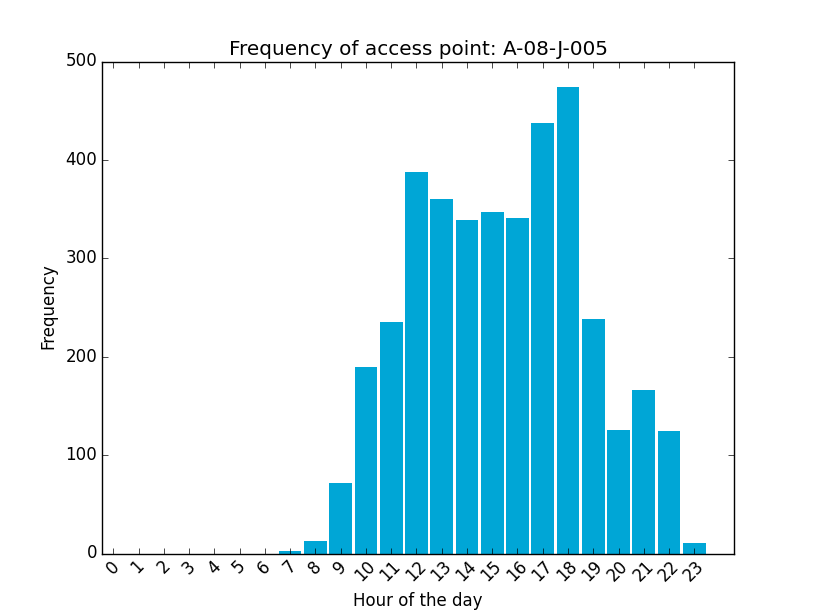
\includegraphics[scale=0.5]{exits_frequency_secondapproach}
\captionsetup{justification=centering}
\caption{Frequency of entrance access point A-08-J-005
}
\label{figure:A-08-J-005Exit}
\end{figure}

The chart shows three interesting peaks, which is in line with what we expected. The first one, around 12am to 1pm, is due to people that leave the building, most probably for lunch. The second peak, around 6pm to 7pm, is due to people that go home for diner. The last one, around 9pm to 10pm, is due to the closing time of the building.

\section{Association rules} 
% Balazs

When a trajectory is simplified into a set of distinct buildings that the person
visited, association rules for buildings can be derived. In this case the rule
describes the set of buildings, or buildingset, that are commonly visited in
combination. For example the rule \{BK\_City, Aula\} \verb|=>| \{Library\}
tells that a group of people who visited the buildings BK\_City and Aula also
visited the Library.

As association rule mining does not consider the order of buildings, nor the
time spent in a building, it is important that these variables are appropriately
handled and noise is filtered out prior running the algorithm.

In the first version the buildingsets were stored in a table as below, where the
field \textit{mac} contains the mac-address of a device and each remaining field
represents a building. Value 1 is given if the device was recorded in a
building, otherwise no value is given. This binary encoding is rather simplistic
as it does not consider the amount of time spent in a building and therefore it
does not allow to differentiate between occasional or regular visits.

\begin{table}[H]
\centering
\captionsetup{justification=centering}
\caption{uncategorized buildingset table}
\label{uncategorized buildingset table}
\begin{tabular}{lllllll}
\cline{1-7}
mac & aula & bk\_city & bouwcampus & btud & ctig & ... \\ \cline{1-7}
A   & 1	& 1    	&        	&  	& 1	& 	\\
B   &  	&      	& 1      	& 1	&  	& 	\\
C   &  	& 1    	&        	&  	& 1	& 	\\
D   & 1	&      	&        	&  	&  	& 	\\
E   & 1	&      	& 1      	&  	&  	& 	\\ \cline{1-7}
\end{tabular}
\end{table}

Therefore in the second version a distinction between \textit{occasional,
regular} and \textit{frequent} stays was added to the buildingsets. The division
between the categories is based on the 40 hour workweek and 1.5 hour lecture
durations (see \autoref{table:stay duration categories}). 

\begin{table}[H]
\centering
\captionsetup{justification=centering}
\caption{Stay duration categories}
\label{table:stay duration categories}
\begin{tabular}{lll}
\cline{1-3}
Category   & hours/week           	& ID \\ \cline{1-3}
occasional & $\leq 0.5$             	& 1  \\
regular	& $\textgreater 0.5, \leq 5$ & 2  \\
frequent   & $\textgreater 5$       	& 3
\end{tabular}
\end{table}

The trajectories of approximately 14,000 devices were used to create the first set of association rules with categorized stay duration. At this stage only the noise was filtered from the data but not the stationary devices, and people carrying two devices were not accounted for. The time range of trajectories spanned from 31.03.2016 to 02.05.2016, approximately one month.

Although there are several measures to evaluate the interestingness of an association rule \parencite{zhang_survey_2009}, only \textit{support} and \textit{confidence} were used for testing purposes. 

\textbf{Support}
“The support for a rule is defined to be the fraction of transaction in the dataset that satisfy the union of items in the consequent and antecedent of the rule.” \parencite{agrawal_mining_1993}. In case of the rule \{BK\_City, Aula\} \verb|=>| \{Library\}, the support is the percentage of the total dataset that includes BK\_City, Aula and Library.

\textbf{Confidence}
Confidence measures the strength of the rule, and is considered as a conditional probability. In case of the rule \{BK\_ City, Aula\} \verb|=>| \{Library\}, the confidence is the probability that Library is in the trajectory if both BK\_ City and Aula are in the trajectory (\cite{agrawal_mining_1993}; \cite{anbukkarasy_interesting_2013}).

The most interesting rules are displayed in \autoref{figure:buildingset}:
\begin{figure}[H]
\centering
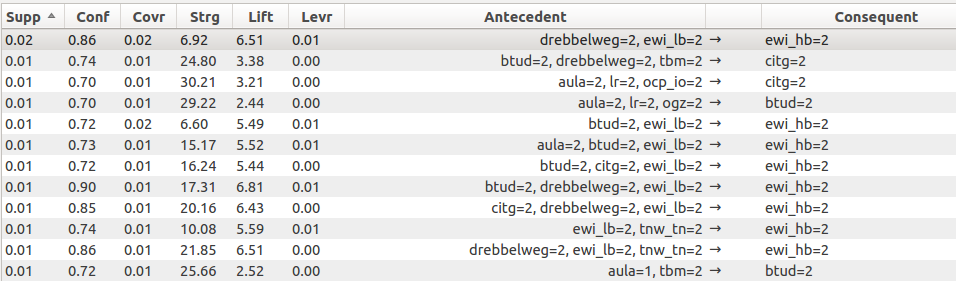
\includegraphics[scale=0.45]{acc_buildingset_v0516}
\captionsetup{justification=centering}
\caption{Building set}
\label{figure:buildingset}
\end{figure}

In the buildingset of approx. 14,000 devices 2\% was recorded in all of the buildings \textit{Drebbelweg, EWI-LB, EWI-HB} (Support = 0.02). There is an 86\% chance that if a device is recorded in the buildings \textit{Drebbelweg, EWI-LB}, then it is also recorded in \textit{EWI-HB} (Confidence = 0.86). And they spent on average between half hour to five hours a week in each building (drebbelweg=2, ewi\_ lb=2, ewi\_ hb=2).

\section{Distinguishing user groups}
% Simon
% People moving in groups

\section{Occupancy}
% Matthijs

\section{AP system}
% Matthijs
% Scan time, also outdoors maybe?

\section{Data reasoning}
% Matthijs evt Simon
% Trajectories

\section{Visual exploration}
% Ethan/Matthijs
% What did and didnt work